\section{Durchführung}
\label{sec:Durchführung}
\subsection{Messung im niedrigen Druckbereich bis $\SI{1}{\bar}$}
Um die Dampfdruckkurve im Druckbereich bis zu $\SI{1}{\bar}$ zu messen, wird die
in Abbildung \ref{fig:messapparatur1} dargestellte Messapparatur verwendet.
\begin{figure}
  \centering
  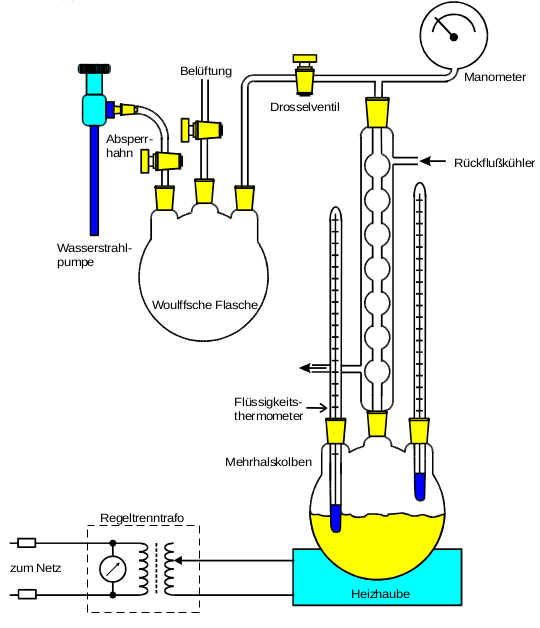
\includegraphics[width=0.6\textwidth]{messapparatur1.png}
  \caption{Schematische Darstellung der Messapparatur für den niedrigen
  Druckbereich \cite{sample}.}
  \label{fig:messapparatur1}
\end{figure}
Diese wird zunächst mit der Wasserstrahlpumpe evakuiert. Dazu wird das
Belüftungsventil geschlossen und der Absperrhahn sowie das Drosselventil geöffnet.
Die Woulffsche Flasche sorgt dafür, dass kein kaltes Wasser in die erhitzte und
evakuierte Glasapparatur gezogen werden kann. Vor dem Abstellen der Wasserstrahlpumpe
muss auf jeden Fall der Absperrhahn geschlossen werden. Das Wasser in dem
Mehrhalskolben wird mit der Heizhaube zum Sieden gebracht, gleichzeitig wird die
Kühlwasserzufuhr für den Rückflusskühler eingeschaltet, sodass der Dampf immer
kondensiert, bevor er in den Manometer gelangen könnte. Sobald die Flüssigkeit
siedet, werden Messwertpaare aus Druck und Temperatur aufgenommen, bis der Druck
ein Bar erreicht hat. Die Temperatur wird dabei an dem Thermomenter abgelesen,
das sich im Dampf befindet.

\subsection{Messung im hohen Druckbereich von $\SI{1}{\bar}$ bis $\SI{15}{\bar}$}
Die Messung für die Dampfdruckkurve im Druckbereich von $\SI{1}{\bar}$ bis
$\SI{15}{\bar}$ wird mit einer Messapparatur wie in Abbildung \ref{fig:messapparatur2}
durchgeführt.
\begin{figure}
  \centering
  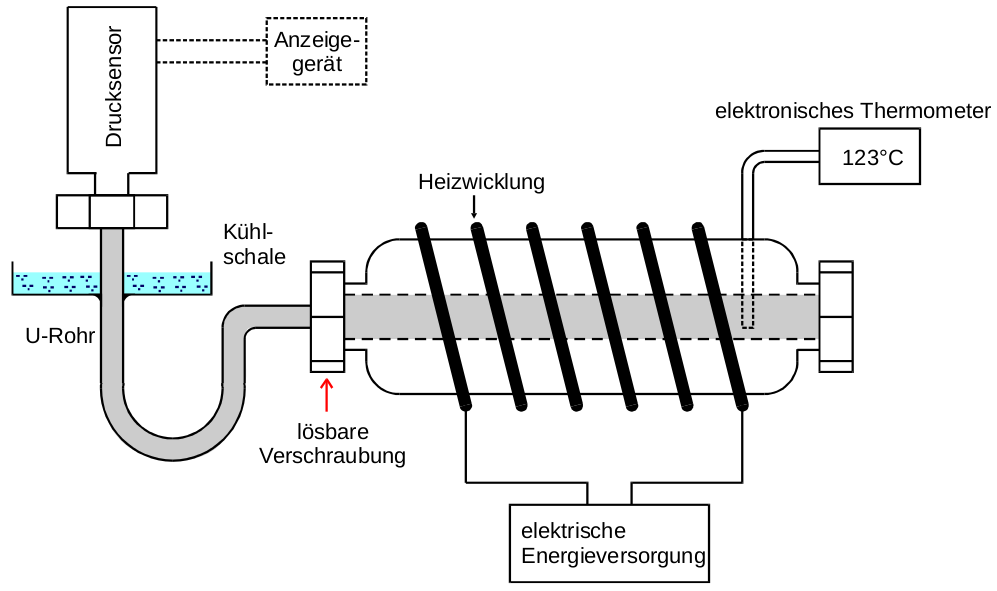
\includegraphics[width=0.7\textwidth]{messapparatur2.png}
  \caption{Schematische Darstellung der Messapparatur für den hohen
  Druckbereich \cite{sample}.}
  \label{fig:messapparatur2}
\end{figure}
Der Hohlraum des Stahlbolzens ist mit Wasser gefüllt. An den Hohlraum ist ein
U-Rohr mit Manometer angeschlossen. Ein Thermometer misst die Temperatur außerhalb
des Hohlraums an der Heizwickelung. Das Wasser wird langsam erhitzt und es werden
Messwertpaare von Temperatur und Druck im Temperaturbereich von $\SI{100}{\celsius}$
bis $\SI{126}{\celsius}$ aufgenommen.
